%%%%%%%%%%%%%%%%%%%%%%%%%%%%%%%%%%%%%%%%%%%%%%%%%%%%%%%%%%%%%%%%%%%%%%%%%%%%%%%%
%2345678901234567890123456789012345678901234567890123456789012345678901234567890
%        1         2         3         4         5         6         7         8

\documentclass[letterpaper, 10 pt, conference]{ieeeconf}  % Comment this line out
                                                          % if you need a4paper
%\documentclass[a4paper, 10pt, conference]{ieeeconf}      % Use this line for a4
                                                          % paper

\IEEEoverridecommandlockouts                              % This command is only
                                                          % needed if you want to
                                                          % use the \thanks command
\overrideIEEEmargins
% See the \addtolength command later in the file to balance the column lengths
% on the last page of the document



% The following packages can be found on http:\\www.ctan.org
%\usepackage{graphics} % for pdf, bitmapped graphics files
%\usepackage{epsfig} % for postscript graphics files
%\usepackage{mathptmx} % assumes new font selection scheme installed
%\usepackage{times} % assumes new font selection scheme installed
\usepackage{amsmath} % assumes amsmath package installed
\usepackage{amssymb}  % assumes amsmath package installed
\usepackage{boldline}
\usepackage{array,multirow}
\usepackage{dblfloatfix} 
\usepackage{hyperref}
\usepackage{float}
\usepackage{color}
\usepackage{xfrac}
\usepackage{graphicx}
\graphicspath{ {images/} }
\definecolor{light-gray}{gray}{0.95}
\newcommand{\code}[1]{\colorbox{light-gray}{\texttt{#1}}}
\DeclareMathOperator*{\argmax}{arg\,max}
\DeclareMathOperator*{\maxU}{max}
\usepackage{makecell}
\usepackage{bbm}
\usepackage[table,xcdraw]{xcolor}
\usepackage[flushleft]{threeparttable}
\usepackage[utf8]{inputenc}
\usepackage{capt-of}


\title{\LARGE \bf
Image Classification With EMNIST - An Extended Version of MNIST
}

\author{ \parbox{2 in}{\centering Tamir Bennatan
         {\tt\small tamir.bennatan@mail.mcgill.ca\\}
         {\tt\small 260614526}}
         \hspace*{ 0.3 in}
         \parbox{2 in}{\centering Kyle Levy
         {\tt\small kyle.levy@mail.mcgill.ca\\}
         {\tt\small 260612028}}
         \hspace*{0.3 in}
         \parbox{2 in}{\centering Phillip Ryjanovsky
         {\tt\small Philip.ryjanovsky@mail.mcgill.ca\\}
         {\tt\small 260604024}}
}


\begin{document}



\maketitle
\thispagestyle{empty}
\pagestyle{empty}


%%%%%%%%%%%%%%%%%%%%%%%%%%%%%%%%%%%%%%%%%%%%%%%%%%%%%%%%%%%%%%%%%%%%%%%%%%%%%%%%


%%%%%%%%%%%%%%%%%%%%%%%%%%%%%%%%%%%%%%%%%%%%%%%%%%%%%%%%%%%%%%%%%%%%%%%%%%%%%%%%
\section{INTRODUCTION}

The MNIST dataset - comprising of images of handwritten digits of 10 classes - is a popular dataset, widely used as a  benchmark for learning and classification tasks amongst the Neural Network and Computer Vision communities. MNIST enjoys several favorable charactaristics which have contributed to its widspread adoption (Cohen, et. al; 2017). First, the dataset is relatively small (each of the 60,000 examples are $(28\text{x}28)$ pixel grayscale images), which makes it feasible to work with the dataset on most processors [Figure 1]. Second, the digits have been centered within each image, have consistent heights and similiar widths. The digits are all distinguishable to the human eye, and the labels associated with each image are accurate. Because of these properties, many reserachers have achived near perfect accuracy in the image classification task on MNIST (for example: Lecun et. al; 2001).

\begin{figure*}[ht]
\centering
\begin{minipage}{.5\textwidth}
  \centering
  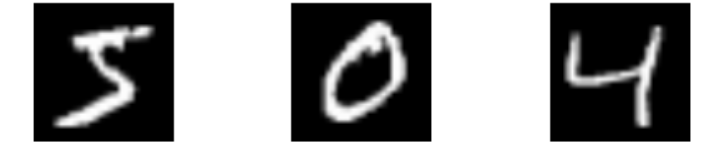
\includegraphics[width=1\linewidth]{mnist_sample}
  \captionof{figure}{Three sample images from the MNIST dataset.}
  \label{fig:test1}
\end{minipage}%
\begin{minipage}{.5\textwidth}
  \centering
  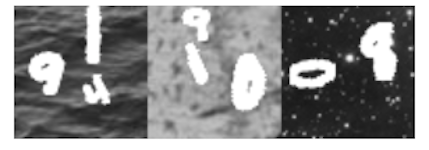
\includegraphics[width=1\linewidth]{emnist_sample}
  \captionof{figure}{Three sample images from the EMNIST dataset.}
  \label{fig:test2}
\end{minipage}
\end{figure*}

In this project, we address the digit classification task on a more difficult dataset called Extended-MNIST (EMNIST). Each example int he EMNIST daset was generated with the following procedure:
\begin{enumerate}
\item Randomly select 2 or 3 images from MNSIT.
\item Rescale each image by a factor ranging from 40\% to 120\% the original size (the label of the generated image is that of the MNIST image which was scaled up by the largest factor).
\item Apply random rotations to each image. 
\item Superimpose these rotated images onto a random background.
\end{enumerate}

The inherent randomness in the EMNIST examples makes image classification on EMNIST more difficult than on MNIST [Figure 2]. 

In this report, we discuss the pre-processing measures we took to adress the noisy features of the EMNIST examples. We then summarize our process in fitting and tuning Logistic Regression, Feedforward Neural Network, and Convolutional Neural Network (CNN) classifiers. CNNs proved most effective; we achieved 92.6\% validation accuracy using the aggregated predictions of four CNN models. We then summarize our results and our shortcomings, and ways in which we can improve our accuracy in the future. 

\section{Feature Design}

The EMNIST dataset introduces several difficulties in building an effective classifier. The random backgrounds of each example in the EMNIST dataset were generated independently of the examles' labels. Thus, they only add noise to each image, which can impede effective learning by a machine learning algorithm. 

It is also unclear which digit in each image was scaled up the most during the construction of each example in EMNIST, as we do not have prior knowledge of the dimension sof the MNIST digits used to create each example in EMNIST. This makes it difficult to isolate the digit within each EMNIST example that corresponds with the target label.

Finally, an effective classifier for the EMNIST dataset must be robust to rotations in images, as the EMNIST datsset was built by rotating MNIST images randomly. As most machine learning algorithms do not encode images in a way that is robust to rotations, this adds diffulty to the classification task. 

\subsection{Removing Noisy Backgrounds} 

The first preprocessing step we took was to remove the backgrounds of each example in EMNIST. Luckily, the pixels in each example corresponding to a digit extracted from MNIST have a fixed integer value of 255 (corresponding to the color white). This made it possible to replace the random backgrounds with black backgrounds, by converting all non-white pixels to black pixel values [Figure 3].
\begin{figure}[H]
      \centering
      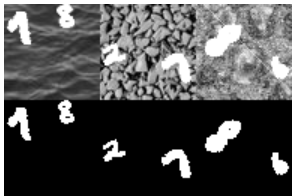
\includegraphics[scale = 1]{blackout}
		\centering
      %\includegraphics[scale=1.0]{figurefile}
      \caption{Three sample images from EMNIST, before filling the backgrounds (top) and after filling the backgrounds (bottom).}
      \label{figurelabel}
   \end{figure}

\subsection{Extracting the 'Largest' Digit} 

Each example in EMNIST contains several digits, but only one label. Intuitively, this makes the learning task difficult, as a machine learning algorithm will try associate the properties of several digits which an example's label, when in fact the task is to only correctly identify the \emph{largest} digit. 

Thus, we set out to extract the \emph{"largest"} digit from each example in EMNIST. Since we do not know the original dimensions of each of the digits in each image, we employed a series of heuristics to define the size of an digit. These heuristics are:
\begin{enumerate}
\item \textbf{Bounding Rectangle Area:} The area of the smallest upright rectangle that circumscribes the digit. 
\item \textbf{Bounding Circle Area:} The area of the smallest circle which escribes the digit. 
\item \textbf{Minimum Rotated Rectangle Area:} The area of the smallest (possibly rotated) rectangle that escribes the digit.
\item \textbf{Minimum Rotated Rectangle Maximum Dimension} The largest dimension (height,width) of the smallest (possibly rotated) rectangle that circumscribes the digit. 
\end{enumerate}
We refer to these huristics as \emph{heuristics 1-4}, respectively.

\begin{figure}[H]
      \centering
      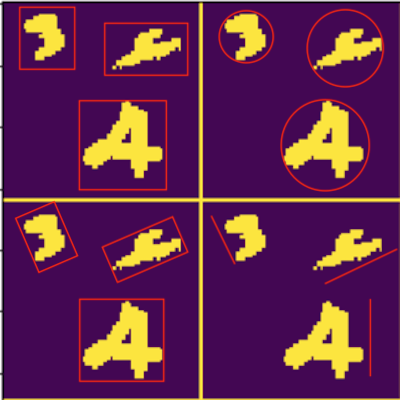
\includegraphics[scale = 1]{size_definitions}
		\centering
      %\includegraphics[scale=1.0]{figurefile}
      \caption{A sample image from EMNIST, superimposed by the geometric objects used to measure the size of each image using heuristics 1-4. Heuristic 1 is the top left, Huerustic 2 is the top right, Heuristic 3 is the bottom left, and Heuristic 4 is the bottom right.}
      \label{figurelabel}
   \end{figure}

We treated the choice of which heuristic to use to measure the size of a digit as a hyperparameter, selected from them using cross-validation. Once we selected a heuristic, cropped each example to the a square which circumscribes the largest digit (according to this heuristic), and resized this square to 28 by 28 pixels. 

\subsection{Data Augmentation} 

To help make our model more robust to rotated digits, we augmented our training data with randomly rotated copies of each training example. Our rational is that if we train on randomly rotated images, our classifier will scale unseen randomly rotated images more effeciely. We tuned the number of times we rotated each image (called the \emph{"batch size"}), and the range of degrees with which we rotated each image as hyperparameters. 


\section{ALGORITHMS}

We trained classifiers of three types: Regularized Logistic Regression, Feedforward Neural Network, and Convolutional Neural Networks (CNN). We trained each of these classifiers on the datasets processed using each of size heuristics described above, though we only experimented with data augmentation when training the CNN.

Regularized Logisitc regression served as our benchmark, as it is a simple and easy to implement algorithm. 

\textbf{THIS IS FILLER. HERE WE TALK A BIT ABOUT IMPLEMENTATION AND WHAT WE TUNEDTHIS IS FILLER. HERE WE TALK A BIT ABOUT IMPLEMENTATION AND WHAT WE TUNEDTHIS IS FILLER. HERE WE TALK A BIT ABOUT IMPLEMENTATION AND WHAT WE TUNEDTHIS IS FILLER. HERE WE TALK A BIT ABOUT IMPLEMENTATION AND WHAT WE TUNEDTHIS IS FILLER. HERE WE TALK A BIT ABOUT IMPLEMENTATION AND WHAT WE TUNEDTHIS IS FILLER. HERE WE TALK A BIT ABOUT IMPLEMENTATION AND WHAT WE TUNEDTHIS IS FILLER. HERE WE TALK A BIT ABOUT IMPLEMENTATION AND WHAT WE TUNED.}

Finally, we trained CNNs of four different archetecutres - each inspired by the LeNet archetecture by Lecun et. al (Legun et. al; 1995). These archetectures alternate between convolutional and max-pooling layers, and output predictions through two fully connected layers. One archetecture had three convolutional layers, two had four convolutional layers, and one had six convolutional layers. 
\begin{figure}[H]
      \centering
      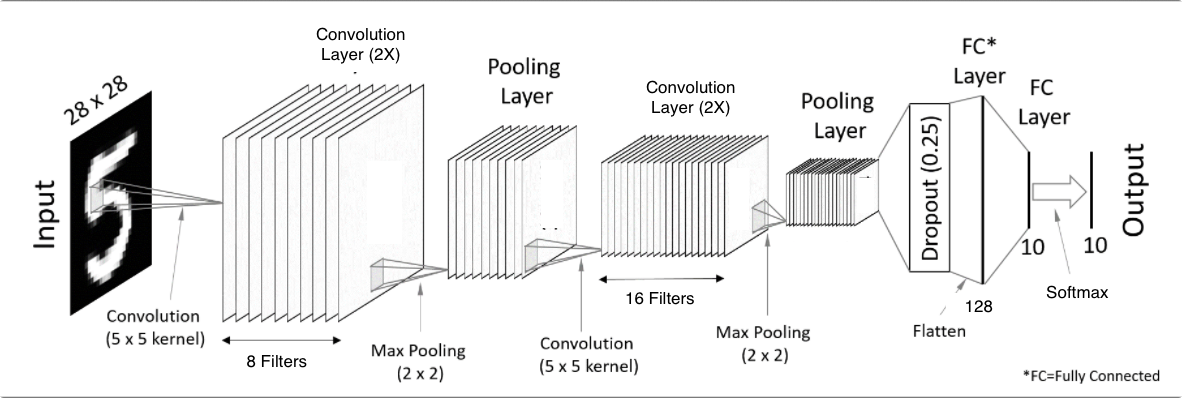
\includegraphics[scale = .42]{conv4_arch}
		\centering
      %\includegraphics[scale=1.0]{figurefile}
      \caption{One of the four CNN archetectures we experimented with. The other three differ slightly in the kernel size, pooling size, and number of convolutional layers. Image modified from [4]. }
      \label{figurelabel}
\end{figure}
A summary of the four architechtures we experimented with is presented in the apenndix. We refer to them as \emph{Architecture 1-4}. 

\section{METHODOLOGY}

We started by splitting the labeled data into training and validation splits of sizes 40,000 and 10,000 examples, respectively. We kept these splits consistent in all experiments, so that we could guage the relative effectiveness of the models. For each model, we used this validation set to select a digit size heuristic, based on which heuristic(s) yield the highest validation accuracy when used to select the largest digit. We also used this validation set to tune model-specific parameters.

\subsection{Logistic Regression: Model Tuning} 

The two hyperparamters we tuned the for logistic regression were the inverse-regularization coefficient, $C$\footnote{In the notation seen in class, $C \propto \sfrac{1}{\lambda}$.}, and the regularization loss function (either \emph{l1} or \emph{l2}). Using the processed datasets generated from using each of the four size heuristics, we ran a grid-search over 24 hyperparameter combinations, and selected the combination that yielded the best validation accuracy.   

\subsection{Feedforward Neural Network: Model Tuning} 

\textbf{THIS IS FILLER. HERE WE TALK A BIT ABOUT IMPLEMENTATION AND WHAT WE TUNEDTHIS IS FILLER. HERE WE TALK A BIT ABOUT IMPLEMENTATION AND WHAT WE TUNEDTHIS IS FILLER. HERE WE TALK A BIT ABOUT IMPLEMENTATION AND WHAT WE TUNEDTHIS IS FILLER. HERE WE TALK A BIT ABOUT IMPLEMENTATION AND WHAT WE TUNEDTHIS IS FILLER. HERE WE TALK A BIT ABOUT IMPLEMENTATION AND WHAT WE TUNEDTHIS IS FILLER.}

\subsection{CNN: Hyperparameter Tuning} 

We considered many hyperparameters when tuning our CNN models. The most important hyperparameters are summarized in Table 1:
\begin{table}[]
\caption{Hyperparameter Ranges Explored for CNN models}
\centering
\label{my-label}
\begin{tabular}{|c|c|}
\hline
\textbf{Hyperparameter}                                                                     & \textbf{Range Explored}                                                                                                            \\ \hline
Model Architecture                                                                          & \begin{tabular}[c]{@{}c@{}}\{Architecture 1, Architecture 2, \\ Architecture 3, Architecture 4\}\end{tabular}                      \\ \hline
\begin{tabular}[c]{@{}c@{}}Data Augmentation - \\ (Batch size, Rotation Range)\end{tabular} & \begin{tabular}[c]{@{}c@{}}\{(1, {[}0, 0{]}), \\ (8, {[}-10, 10{]}), \\ (16, {[}-20, 20{]}), \\ (16, {[}-30, 30{]})\}\end{tabular} \\ \hline
\multicolumn{1}{|l|}{Learning Rate}                                                         & \multicolumn{1}{l|}{\{.000001, .00005, .0001\}}                                                                                  \\ \hline
Digit Size Heuristic                                                                        & \begin{tabular}[c]{@{}c@{}}\{Heuristic 1, Heuristic 2,\\  Heuristic 3, Heuristic 4\}\end{tabular}                                  \\ \hline
\end{tabular}
\end{table}

We started by training all four architectures on the data preprocessed using Heuristic 1 with the high learning rate of $.0001$. After observing that architectures 2 and 4 yielded much higher validation accuracy than architectures 1 and 3, we decided to omit the latter architectures from all further expiriments. We also decided to limit the range of the learning rate $\eta$ to $\eta \in \{.000001, .00005\}$, as we saw that convergence was occuring with high variance.

We then took a random sample of 64 images from EMNIST, and extracted the "largest" digit from each image using each of the four size heuristics defined. We observed by visual inspection that when using Heuristics 3 and 4, we isolated the digits corresponding to the labels more frequently than when we used Heuristics 1 and 2. We decided to use data preprocessed with Heuristics 3 and 4 in all further experiemnts. 

We then performed a gridsearch on the remaining hyperparameter combinations permitted by the constrained hyperparameter ranges [Table 2], totalling paramter combinations.


\begin{table}[]
\centering
\caption{Constrained Hyperparameter Ranges}
\label{my-label}
\begin{tabular}{|c|c|}
\hline
\textbf{Hyperparameter}                                                                     & \textbf{Range Explored}                                                                                                            \\ \hline
Model Architecture                                                                          & \{Architecture 2, Architecture 4\}                                                                                                 \\ \hline
\begin{tabular}[c]{@{}c@{}}Data Augmentation - \\ (Batch size, Rotation Range)\end{tabular} & \begin{tabular}[c]{@{}c@{}}\{(1, {[}0, 0{]}), \\ (8, {[}-10, 10{]}), \\ (16, {[}-20, 20{]}), \\ (16, {[}-30, 30{]})\}\end{tabular} \\ \hline
Learning Rate                                                                               & \{.000001, .00005\}                                                                                                               \\ \hline
Digit Size Heuristic                                                                        & \{Heuristic 3, Heuristic 4\}                                                                                                       \\ \hline
\end{tabular}
\end{table}


\subsection{CNN: Learning Optimization} 

We learned the weights of our networks using the \emph{RMSProp} algorithm, with the hyperparameter $\rho$ fixed at 0.9. While learning, we used an early stopping scheme, which caused training to stop if the validation accuracy has not improved for 8 consecutive epochs. 

At first, we tried learning using learning rate of $\eta = .0001$, but we observed through the use of learning curves that the convergence had very high variance. After reducing the learning rate to $.00005$, we achieved smoother learning [Figure 6].

\begin{figure}
      \centering
      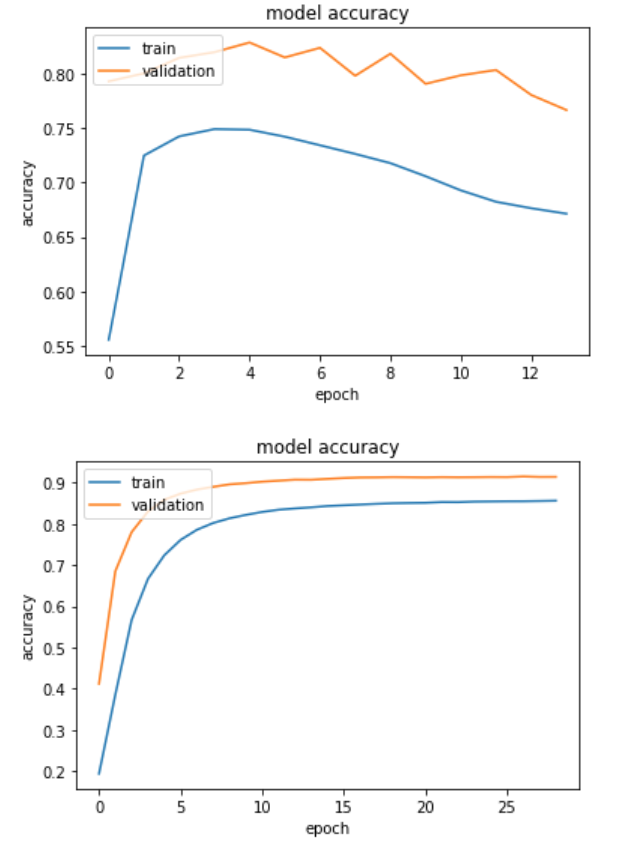
\includegraphics[scale = .6]{learning_curves.png}
		\centering
      %\includegraphics[scale=1.0]{figurefile}
      \caption{Learning curves for training periods with $\eta = .0001$ and $\eta = .00005$, with early stopping. Note: training accuracy is lower than validation accuracy. This is because we used data augmentation, and the new randomly rotated images made the training data "harder" to learn than the validation data.}
      \label{figurelabel}
\end{figure}

\subsection{CNN: Aggregated Predictions} 

We initialized the weights of our CNN's randomly. As such, every time we fit a model with a certain configuration, the final weights may be different, leading to different predictions. 

To account for this randomness, we fit two models of each hyperparameter configuration, each with different random initialization. This allowed us to keep the better of the two trained models (based on validation-set accuracy) for each hyperparameter configuration. 

Thus, for every combination of the hyperparameters (Data Augmentation Strategy, Size Heuristic), we had two models fit using Architecture 2, and two models fit using Architecture 4. This gave us the opportunity to aggregate predictions\footnote{To aggregate predictions of several models, we used the class which was predicted the most frequently amongst each individual model to be the aggregated class prediction.} across several trained models. 

Two of the aggregations we experimented with increased validation accuracy by over 1\%, which we considered substatial. We refer to these aggregations as \emph{Aggregation 1} and \emph{Aggregation 2}. 

\textbf{Aggregation 1:}
\begin{itemize}
\item Predictions of four models aggregated.
\item Two configurations - each repeated once with a different random initialization.
\item Configuration 1: Architechture 2, Batch Bize = 16, Rotation Range [-.2, .2], $\eta$ = .00005, Size Heuristic 3
\item Configuration 2: Architechture 4, Batch Bize = 16, Rotation Range [-.2, .2], $\eta$ = .00005, Size Heuristic 4
\item Configuration 3: Architechture 2, Batch Bize = 16, Rotation Range [-.2, .2], $\eta$ = .00005, Size Heuristic 3
\item Configuration 4: Architechture 4, Batch Bize = 16, Rotation Range [-.2, .2], $\eta$ = .00005, Size Heuristic 4
\end{itemize}
\textbf{Aggregation 2:}
\begin{itemize}
\item The same four configurations as in Aggregation 1, but each model configuration was trained and included twice.
\end{itemize}

\section{RESULTS}

We achieved the highest 


To measure the importance of each of these feature sets, we trained logistic regression and XGB models on all the features described above. We then removed different subsets of Tf-Idf, question classification and semantic scoring feature sets, and re-tuned each model's hyperparameters using 3-fold cross validation. We then used these models to predict test-set labels. The prediction accuracy for the resulting models are summarized in Table 4, as well as those of our baseline classifiers described in section 4.A. We limit our analysis to the XGB model, as this performed much better than logistic regression. 

% Please add the following required packages to your document preamble:
% \usepackage[table,xcdraw]{xcolor}
% If you use beamer only pass "xcolor=table" option, i.e. \documentclass[xcolor=table]{beamer}
\begin{table*}[]
\centering
\caption{Test set accuracy scores, with different feature sets omitted}
\label{my-label}
\begin{threeparttable}
\begin{tabular}{|
>{\columncolor[HTML]{EFEFEF}}l |c|c|c|c|c|c|c|c|}
\hline
\multicolumn{9}{|c|}{\cellcolor[HTML]{ECF4FF}XGB  AND LOGISTIC REGRESSION, WITH FEATURE SETS OMITTED}                                                                                                                                                                \\ \hline
Feature sets ommited                                                            & $\emptyset$    & \{1\}                & \{2\}                & \{3\}                & \{1,2\}       & \{1,3\}                       & \{2,3\}                      & \{1,2,3\}     \\ \hline
XGB Test Set Accuracy                                                           & \textbf{.7925} & .7624 (.0301)        & .7861 (.0064)        & .7825 (.01)          & .7585 (.034)  & .7504 (.0421)                 & .7794 (.0131)                & .7456 (.0469) \\ \hline
\begin{tabular}[c]{@{}l@{}}Logistic Regression\\ Test Set Accuracy\end{tabular} & \textbf{.6962} & .6838 (.0124)        & .6951 (.0011)        & .6837 (.0125)        & .6836 (.0126) & .6743 (.0219)                 & .6827 (.0125)                & .6728 (.0234) \\ \hline
\multicolumn{9}{|c|}{\cellcolor[HTML]{ECF4FF}BASELINE MODELS}                                                                                                                                                                                                        \\ \hline
\multicolumn{1}{|c|}{\cellcolor[HTML]{EFEFEF}Manhattan LSTM}                    & .7588          & \multicolumn{3}{c|}{\cellcolor[HTML]{EFEFEF}Human (400 Responses)} & .8175         & \multicolumn{2}{c|}{\cellcolor[HTML]{EFEFEF}Random Guessing} \& .5015         \\ \hline
\end{tabular}
\begin{tablenotes}
\item Here, \{1\} are the Tf-Idf features from 4.B, \{2\} are the question classification features from 4.C, and \{3\} are the semantic similarity scores from 4.D.
\item Cells contain each model's prediction accuracy, as well as the difference between prediction accuracy and the best model's prediction accuracy. 
\end{tablenotes}
\end{threeparttable}
\end{table*}

\begin{figure*}[t]
\centering
\begin{minipage}{.5\textwidth}
  \centering
  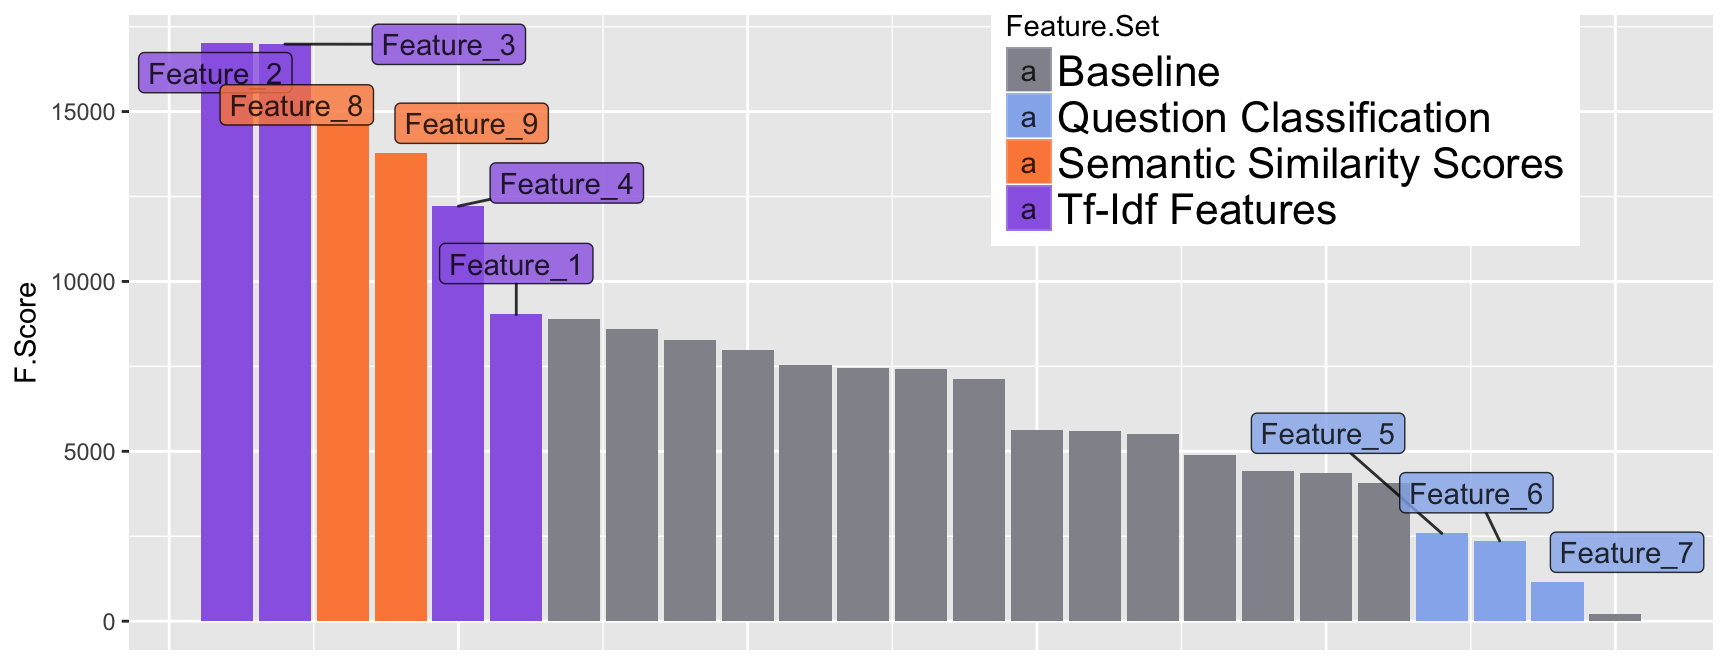
\includegraphics[width=1\linewidth]{full_bars}
  \captionof{figure}{Variable importance chart of model trained on all features.}
  \label{fig:test1}
\end{minipage}%
\begin{minipage}{.5\textwidth}
  \centering
  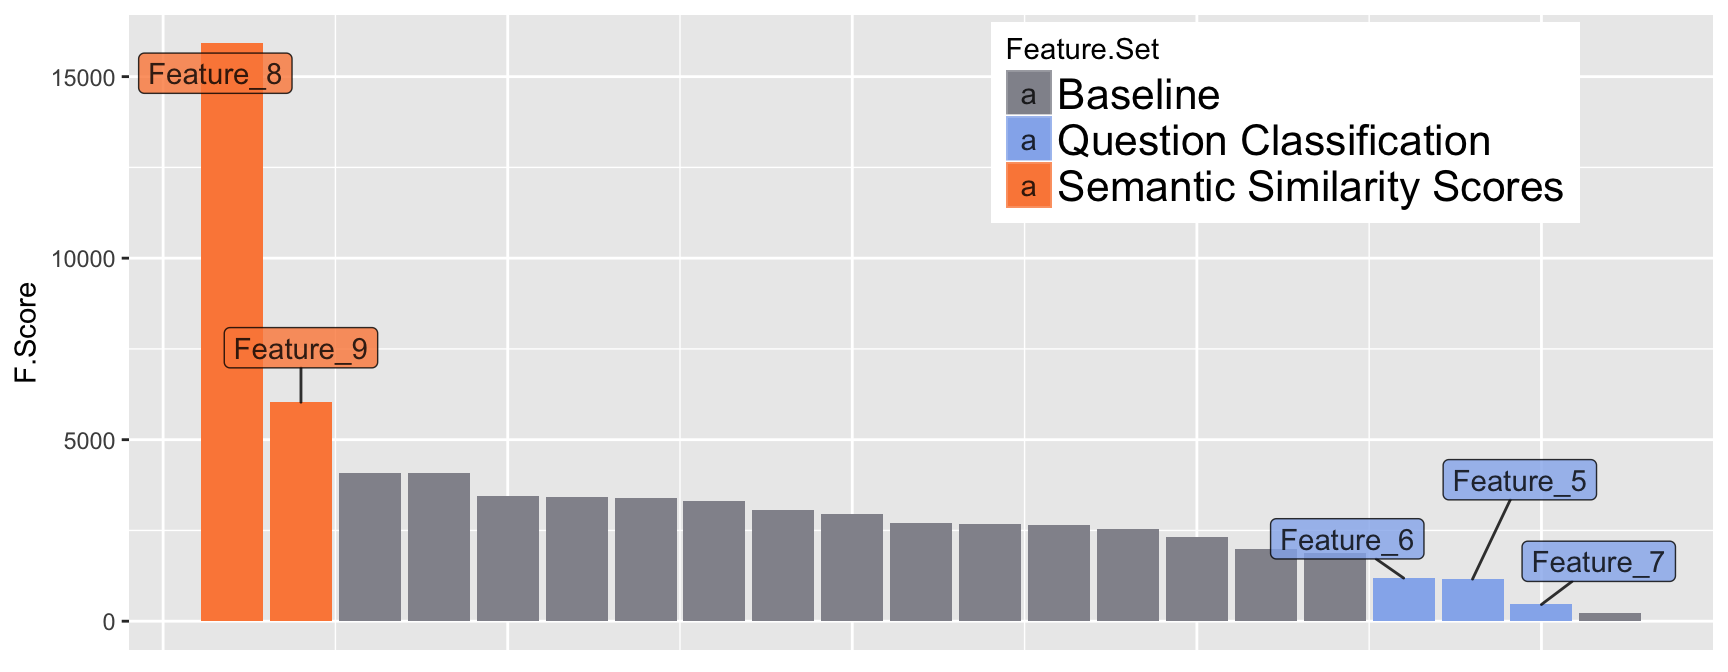
\includegraphics[width=1\linewidth]{no_tfidf_bars}
  \captionof{figure}{Variable importance chart of model that excludes the Tf-Idf features.}
  \label{fig:test2}
\end{minipage}
\end{figure*}

Including all three feature sets results in the best performance, with a test set accuracy of 79.25\% - 4.69\% better than the baseline XGB model. Amongst the three feature sets we propose, removing the Tf-Idf features (4.B) results in the largest decrease in prediction accuracy relative to the full model - with a 3.01\% decrease. Removing the question classification features from 4.C results in the smallest decrease in prediction accuracy, indicating that these features are the least meaningful of those we propose. 

When using ensembled tree models such as XGB, one can use the number of times a variable is split upon as a measure of that variable's importance. This measure is called the \emph{F-Score}. By plotting the F-Scores of each feature, we can gain insight into the importance of each variable used in a model, relative to the other variables present (Gareth et al; 2017).

A variable importance chart of the full model corroborates the result that the Tf-Idf features are the most meaningful, as these features are amongst those with the highest F-Scores [figure 1]. Semantic similarity scores also have high F-Scores. Interestingly, when the Tf-Idf features are removed, the semantic similarity scores become much more important relative to the remaining features, evident in Figure 2. This suggests that the Tf-Idf features and semantic similarity scores explain some of the same variance, and once the Tf-Idf features are removed the model must rely more heavily on the semantic similarity scores. Indeed, the features in these to feature sets are strongly correlated; the correlation between Feature 9 and Features 6 and 7 are 68.28\% and -73.91\%, respectively. 

The variable importance charts also suggest that the question classification features are not meaningful. In fact, these three features are amongst four features with the lowest F-Score.


\section{DISCUSSION AND CONCLUSIONS}

Using the three sets of features described in this paper, we were able to improve the accuracy of our baseline model from 74.56\% to 79.25\%. Of the three feature sets, those computed using Tf-Idf scores were the most impactful. This confirms our hypothesis that measures of word importance and specificity are useful in comparing the semantic similarity between two questions. 

We also applied and extended a framework for modelling semantic similarities between short texts using knowledge-based word similarity scores, proposed by Mihalcea et al (2006). We found that these scores were useful in our classification task. These features were highly correlated with those calculated using Tf-Idf scores, so it may be that they are merely capturing the specificity of the words in each question, rather than the semantic similarity of these words. 

Finally, we found that our answer type predictions were not useful for detecting duplicate questions. We suspect that this is because we used overly complex models to predict the answer type of a question. The TREC dataset has only 6,000 observations, but the number of parameters in our LSTM classifiers ranged from 70,506 to 28,141,268. It's probable that these classifiers were overfit to the TREC dataset, and did not generalize to the Quora dataset. 

In future work, we would like to try using simpler models for predicting a question's answer type - such as Naïve Bayes or a Support Vector Machine. We could also try to incorporate predictions of the fine answer categories in the annotated TREC dataset, as apposed to the coarse categories we used. 

We also think that an interesting extension to this work would be to extract features that concern the grammatical functions of the words in each question. For example, one could construct a dependency parse tree for each question, and compare the subjects and  direct objects in each question, as well as the head words of their repsective parses.

\addtolength{\textheight}{-12cm}   % This command serves to balance the column lengths
                                  % on the last page of the document manually. It shortens
                                  % the textheight of the last page by a suitable amount.
                                  % This command does not take effect until the next page
                                  % so it should come on the page before the last. Make
                                  % sure that you do not shorten the textheight too much.

%%%%%%%%%%%%%%%%%%%%%%%%%%%%%%%%%%%%%%%%%%%%%%%%%%%%%%%%%%%%%%%%%%%%%%%%%%%%%%%%



%%%%%%%%%%%%%%%%%%%%%%%%%%%%%%%%%%%%%%%%%%%%%%%%%%%%%%%%%%%%%%%%%%%%%%%%%%%%%%%%



%%%%%%%%%%%%%%%%%%%%%%%%%%%%%%%%%%%%%%%%%%%%%%%%%%%%%%%%%%%%%%%%%%%%%%%%%%%%%%%%


\section{STATEMENT OF CONTRIBUTION}

Tamir engineered the features and classifiers described, worked on the paper, and conducted model experiments. Jack contributed to the classifiers and paper, and experimented with advanced techniques for feature extraction, such as named entity recognition and headword extraction. 

\section{APPENDIX}
\pagebreak
\begin{figure}
      \centering
      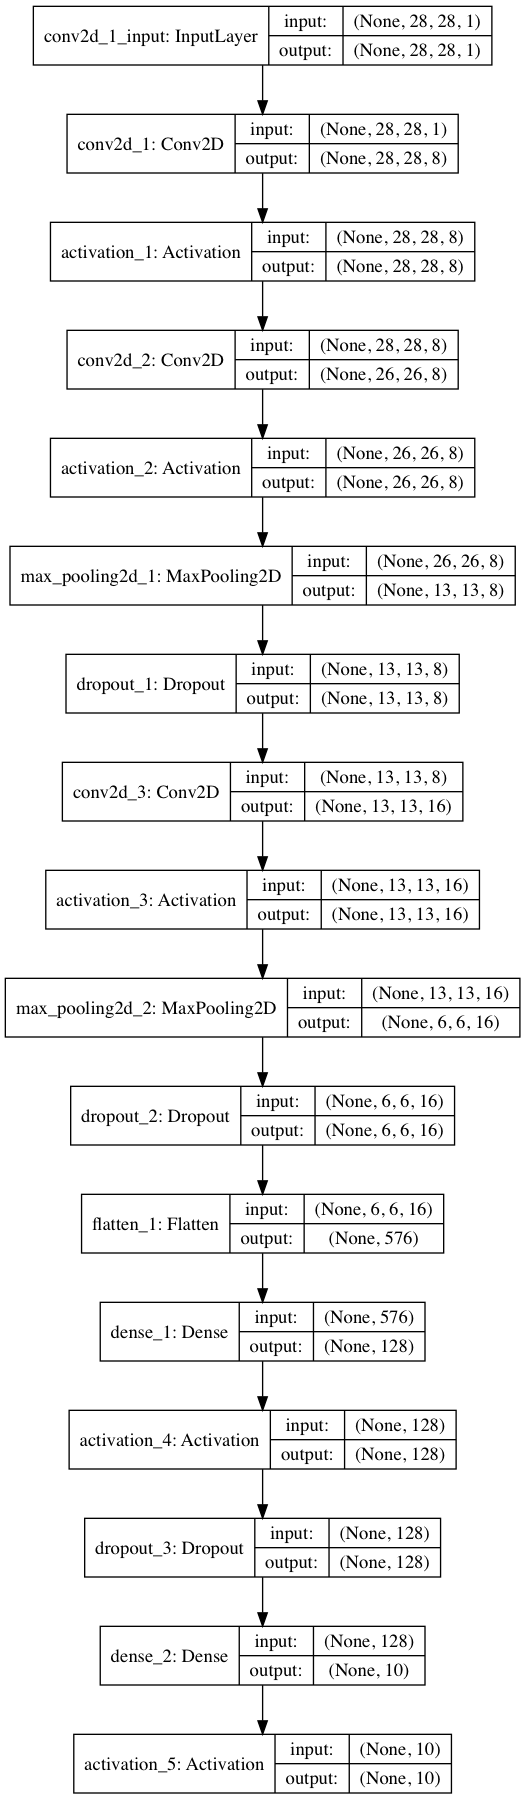
\includegraphics[scale = .35]{model0.png}
		\centering
      %\includegraphics[scale=1.0]{figurefile}
      \caption{Architecture 1: Three convolutional layers, 76,978 trainable parameters.}
      \label{figurelabel}
   \end{figure}
   
\begin{figure}
      \centering
      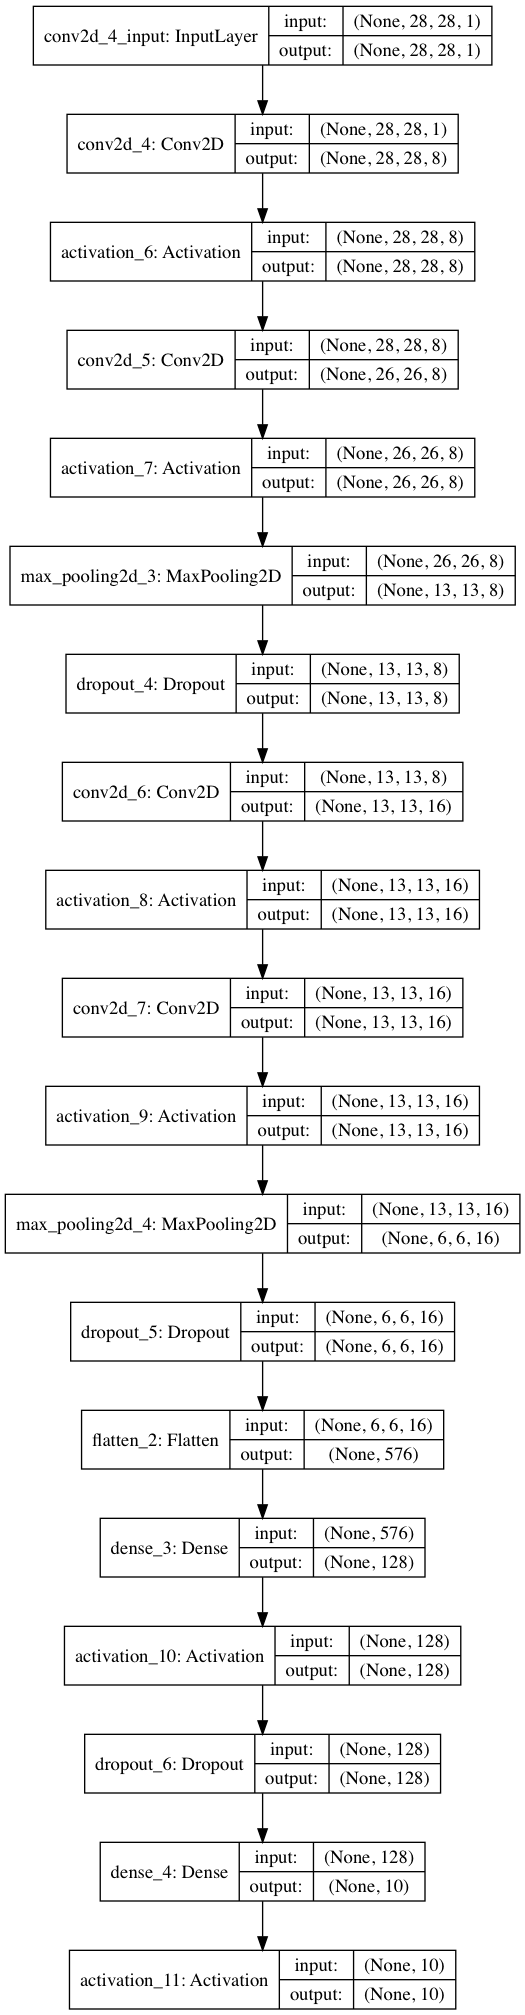
\includegraphics[scale = .3]{model1.png}
		\centering
      %\includegraphics[scale=1.0]{figurefile}
      \caption{Architecture 2: Four convolutional layers, 79,298 trainable parameters.}
      \label{figurelabel}
   \end{figure}
   
\begin{figure}
      \centering
      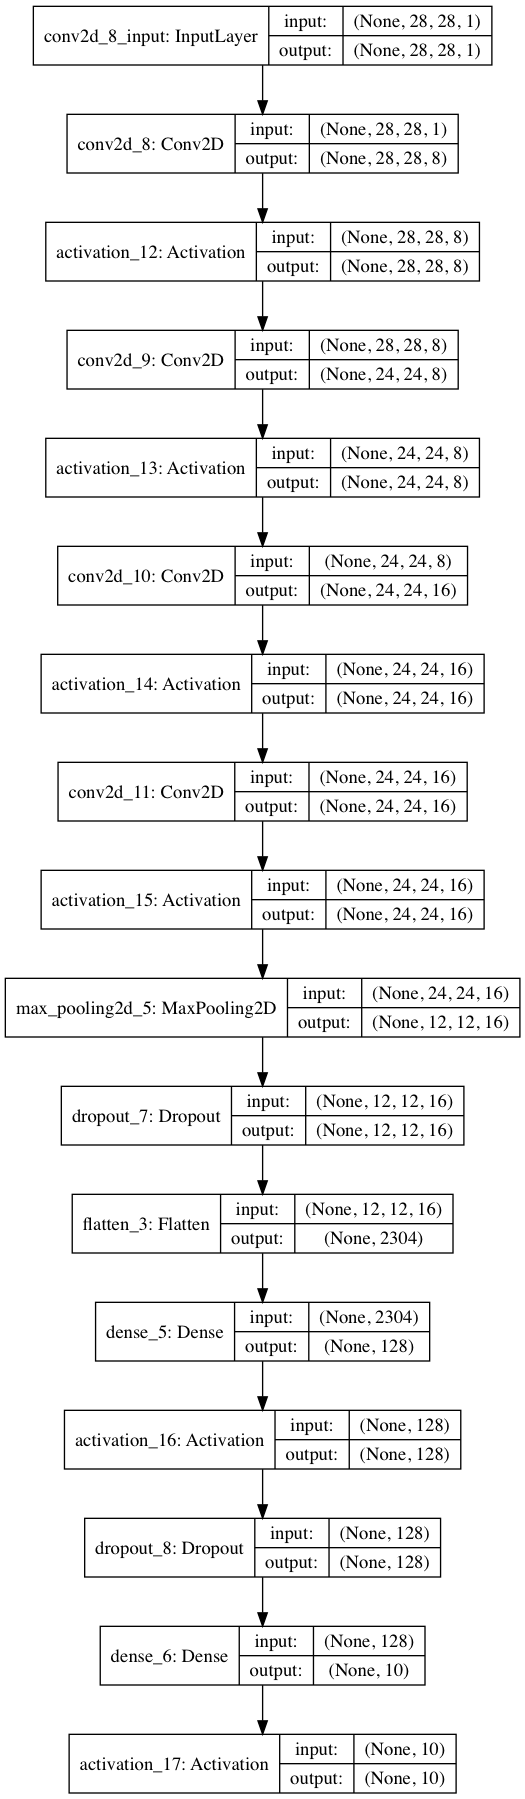
\includegraphics[scale = .3]{model2.png}
		\centering
      %\includegraphics[scale=1.0]{figurefile}
      \caption{Architecture 3: Four convolutional layers, 307,778 trainable parameters.}
      \label{figurelabel}
   \end{figure}
   
\begin{figure}
      \centering
      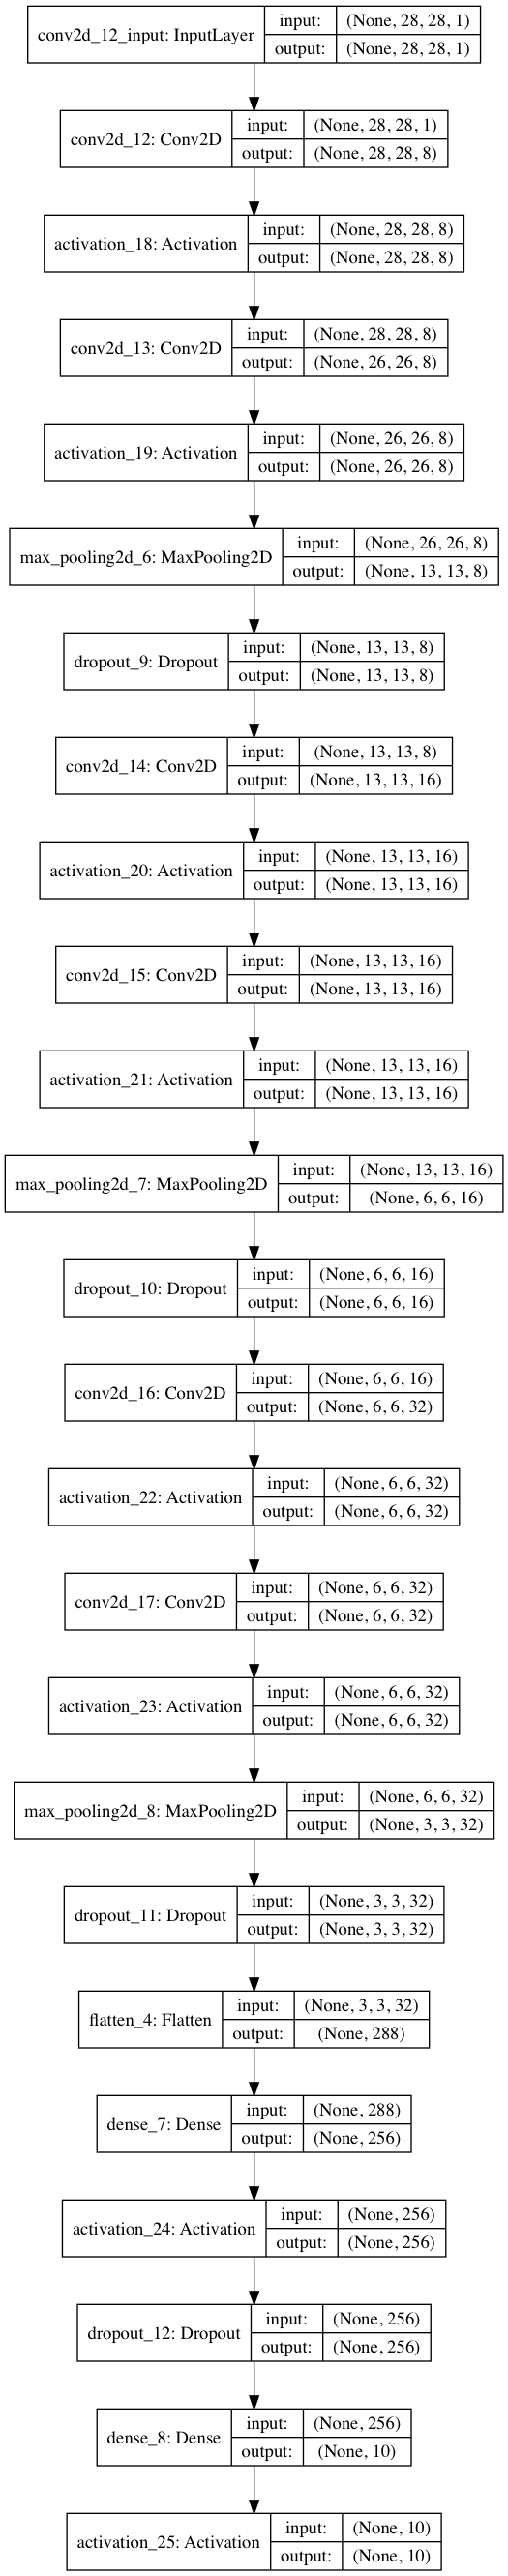
\includegraphics[scale =.2]{model3.png}
		\centering
      %\includegraphics[scale=1.0]{figurefile}
      \caption{Architecture 4: Six convolutional layers, 94,594 trainable parameters.}
      \label{figurelabel}
 \end{figure}


\pagebreak
\begin{thebibliography}{99}
\bibitem{c1} Cohen, G., Afshar, S., Tapson, J., \& van Schaik, A. (2017). EMNIST: an extension of MNIST to handwritten letters. Retrieved from http://arxiv.org/abs/1702.05373 (link is external)
\bibitem{c2} Y. LeCun, L. Bottou, Y. Bengio and P. Haffner: Gradient-Based Learning Applied to Document Recognition, Intelligent Signal Processing, 306-351, IEEE Press, 2001,
\bibitem{c3} Y. LeCun, L. D. Jackel, L. Bottou, A. Brunot, C. Cortes, J. S. Denker, H. Drucker, I. Guyon, U. A. Muller, E. Sackinger, P. Simard and V. Vapnik: Comparison of learning algorithms for handwritten digit recognition, in Fogelman, F. and Gallinari, P. (Eds), International Conference on Artificial Neural Networks, 53-60, EC2 \& Cie, Paris, 1995.


\section*{Blog Posts}

\bibitem{c5} Theart, R. (2017, November 29). Getting started with PyTorch for Deep Learning (Part 3: Neural Network basics). Retrieved from https://codetolight.wordpress.com/2017/11/29/getting-started-with-pytorch-for-deep-learning-part-3-neural-network-basics/

\end{thebibliography}



\end{document}
